\begin{figure}[htbp]
\centering
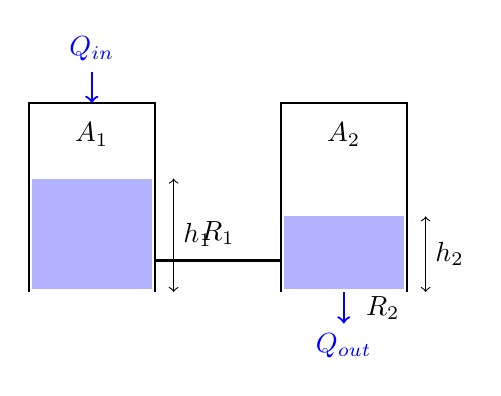
\begin{tikzpicture}[scale=0.8]
    % Tank 1
    \draw[thick] (0,0) -- (0,3) -- (2,3) -- (2,0);
    \fill[blue!30] (0.05,0.05) rectangle (1.95,1.8);
    \node at (1,2.5) {$A_1$};
    \draw[<->] (2.3,0) -- (2.3,1.8) node[midway, right] {$h_1$};

    % Tank 2
    \draw[thick] (4,0) -- (4,3) -- (6,3) -- (6,0);
    \fill[blue!30] (4.05,0.05) rectangle (5.95,1.2);
    \node at (5,2.5) {$A_2$};
    \draw[<->] (6.3,0) -- (6.3,1.2) node[midway, right] {$h_2$};

    % Connecting pipe
    \draw[thick] (2,0.5) -- (4,0.5);
    \node[above] at (3,0.6) {$R_1$};

    % Inflow
    \draw[->, thick, blue] (1,3.5) -- (1,3) node[above, pos=0] {$Q_{\text{in}}$};

    % Outflow
    \draw[->, thick, blue] (5,0) -- (5,-0.5) node[below] {$Q_{\text{out}}$};
    \node[right] at (5.2,-0.25) {$R_2$};
\end{tikzpicture}
\caption{Two interacting tanks.}
\label{fig:two_tanks}
\end{figure}
